\documentclass[12]{article}
\usepackage[utf8]{inputenc}
\usepackage[T2A]{fontenc}
\usepackage[mongolian]{babel}
\usepackage{graphicx}
\graphicspath{ {images/} }
\title{Даалгавар}
\author{B140920764}
\begin{\document}
	\section{Функциональ шаардлага}
	\begin{itemize}
		\item Багш
		\item Оюутны хийх даалгаврыг байршуулах(нэмэх, өөрчлөх)
		\item Оюутны илгээсэн даалгаврыг харах, үнэлгээ өгөх
		\item Оюутан руу хариу илгээх
		\item Оюутны мэдээлэл харах
		\item Даалгавар илгээх, дуусах хугацааг тодорхойлох
		\item Хугацаа хэтэрвэл оноо хасна
		\item Даалгаврыг файл болон текстээр оруулж болно
		\item Тайлан гаргах(дүнгийн дундаж, сэдвийн тайлан)
		\item Оюутан
		\item Багшийн байршуулсан даалгаврыг харах
		\item Даалгавар илгээх(файл болон текстээр) 
		\section{Функциональ бус шаардлага}
		\begin{itemize}
			\item Бүх төрлийн төхөөрөмжид тохиромжтой хэлбэрээр харагддаг/респонсив/ загвартай байна
	\end{itemize}
	\section{Use case diagram}
	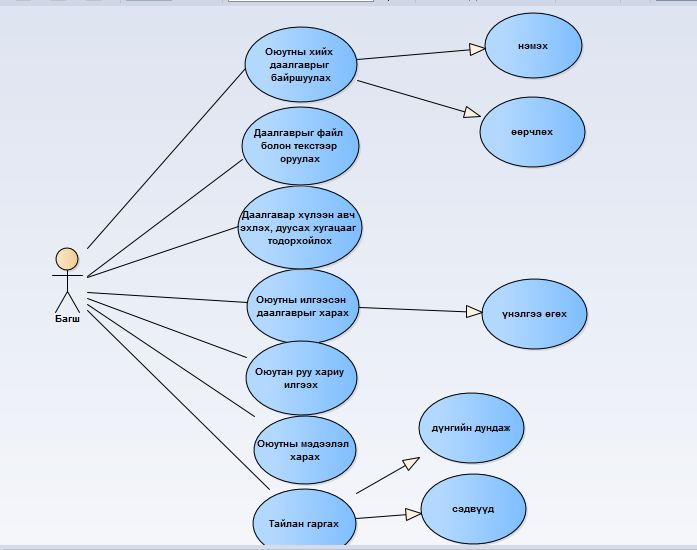
\includegraphics[width=1\textwidth]{images/use-case1.jpg}
	
	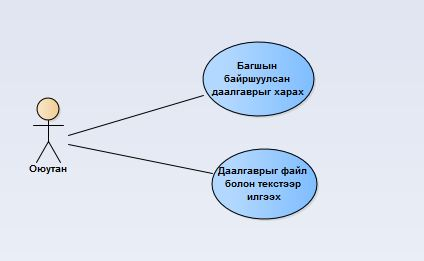
\includegraphics[width=1\textwidth]{images/use-case2.jpg}
	
	\section{Activity diagram(Даалгавар байршуулах)}
	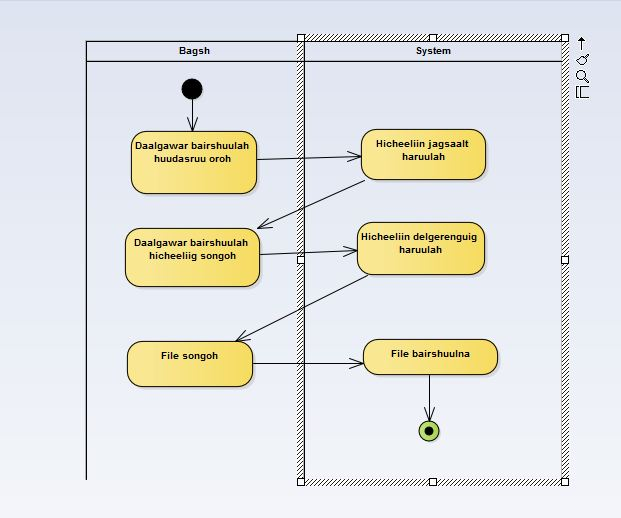
\includegraphics[width=1\textwidth]{images/Daalgawar-bairshuulah-activity}
	
	\section{Даалгавар илгээх}
	\includegraphics[width=1\textwidth]{images/daalgawar-ilgeeh-activity}
	
	\section{Үнэлгээ өгөх}
	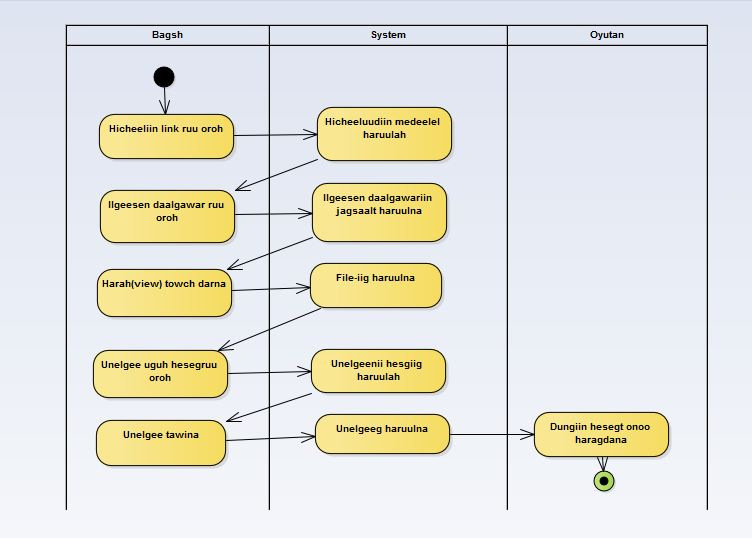
\includegraphics[width=1\textwidth]{images/unelgee-uguh-activity}
	
	\section{Class diagram}
	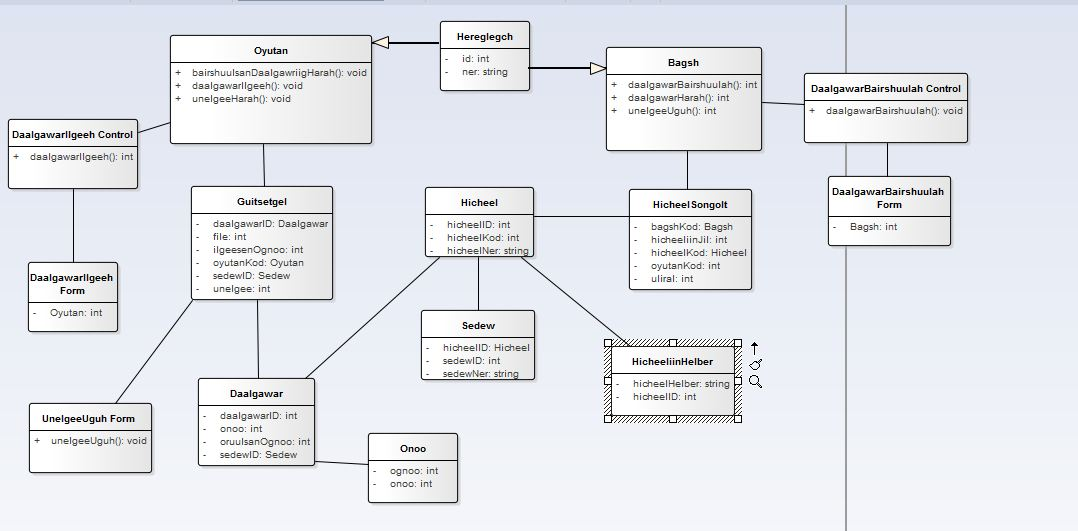
\includegraphics[width=1\textwidth]{images/class-diagram}
	
	\section{Sequence diagram}
	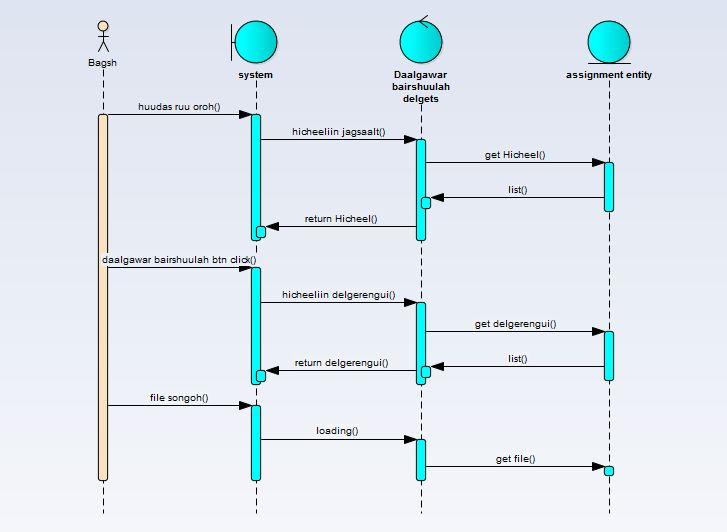
\includegraphics[width=1\textwidth]{images/sequence-diagram}
	
\end{document}
